% Figure: per-species F1 by architecture (small multiples)
% Source   : docs/reports/experiments/phase_1b/final_b_new_recomputed/
%            20260819T043733Z/per_class_metrics.csv
% Artifacts: artifact/person3/per_class/{perclass_f1_summary.csv,
%            perclass_metadata.json, error_analysis.md}
% Run ids  : 15 (5 backbones x seeds 42/123/456), listed in perclass_metadata.json
\begin{figure}[!htbp]
\centering
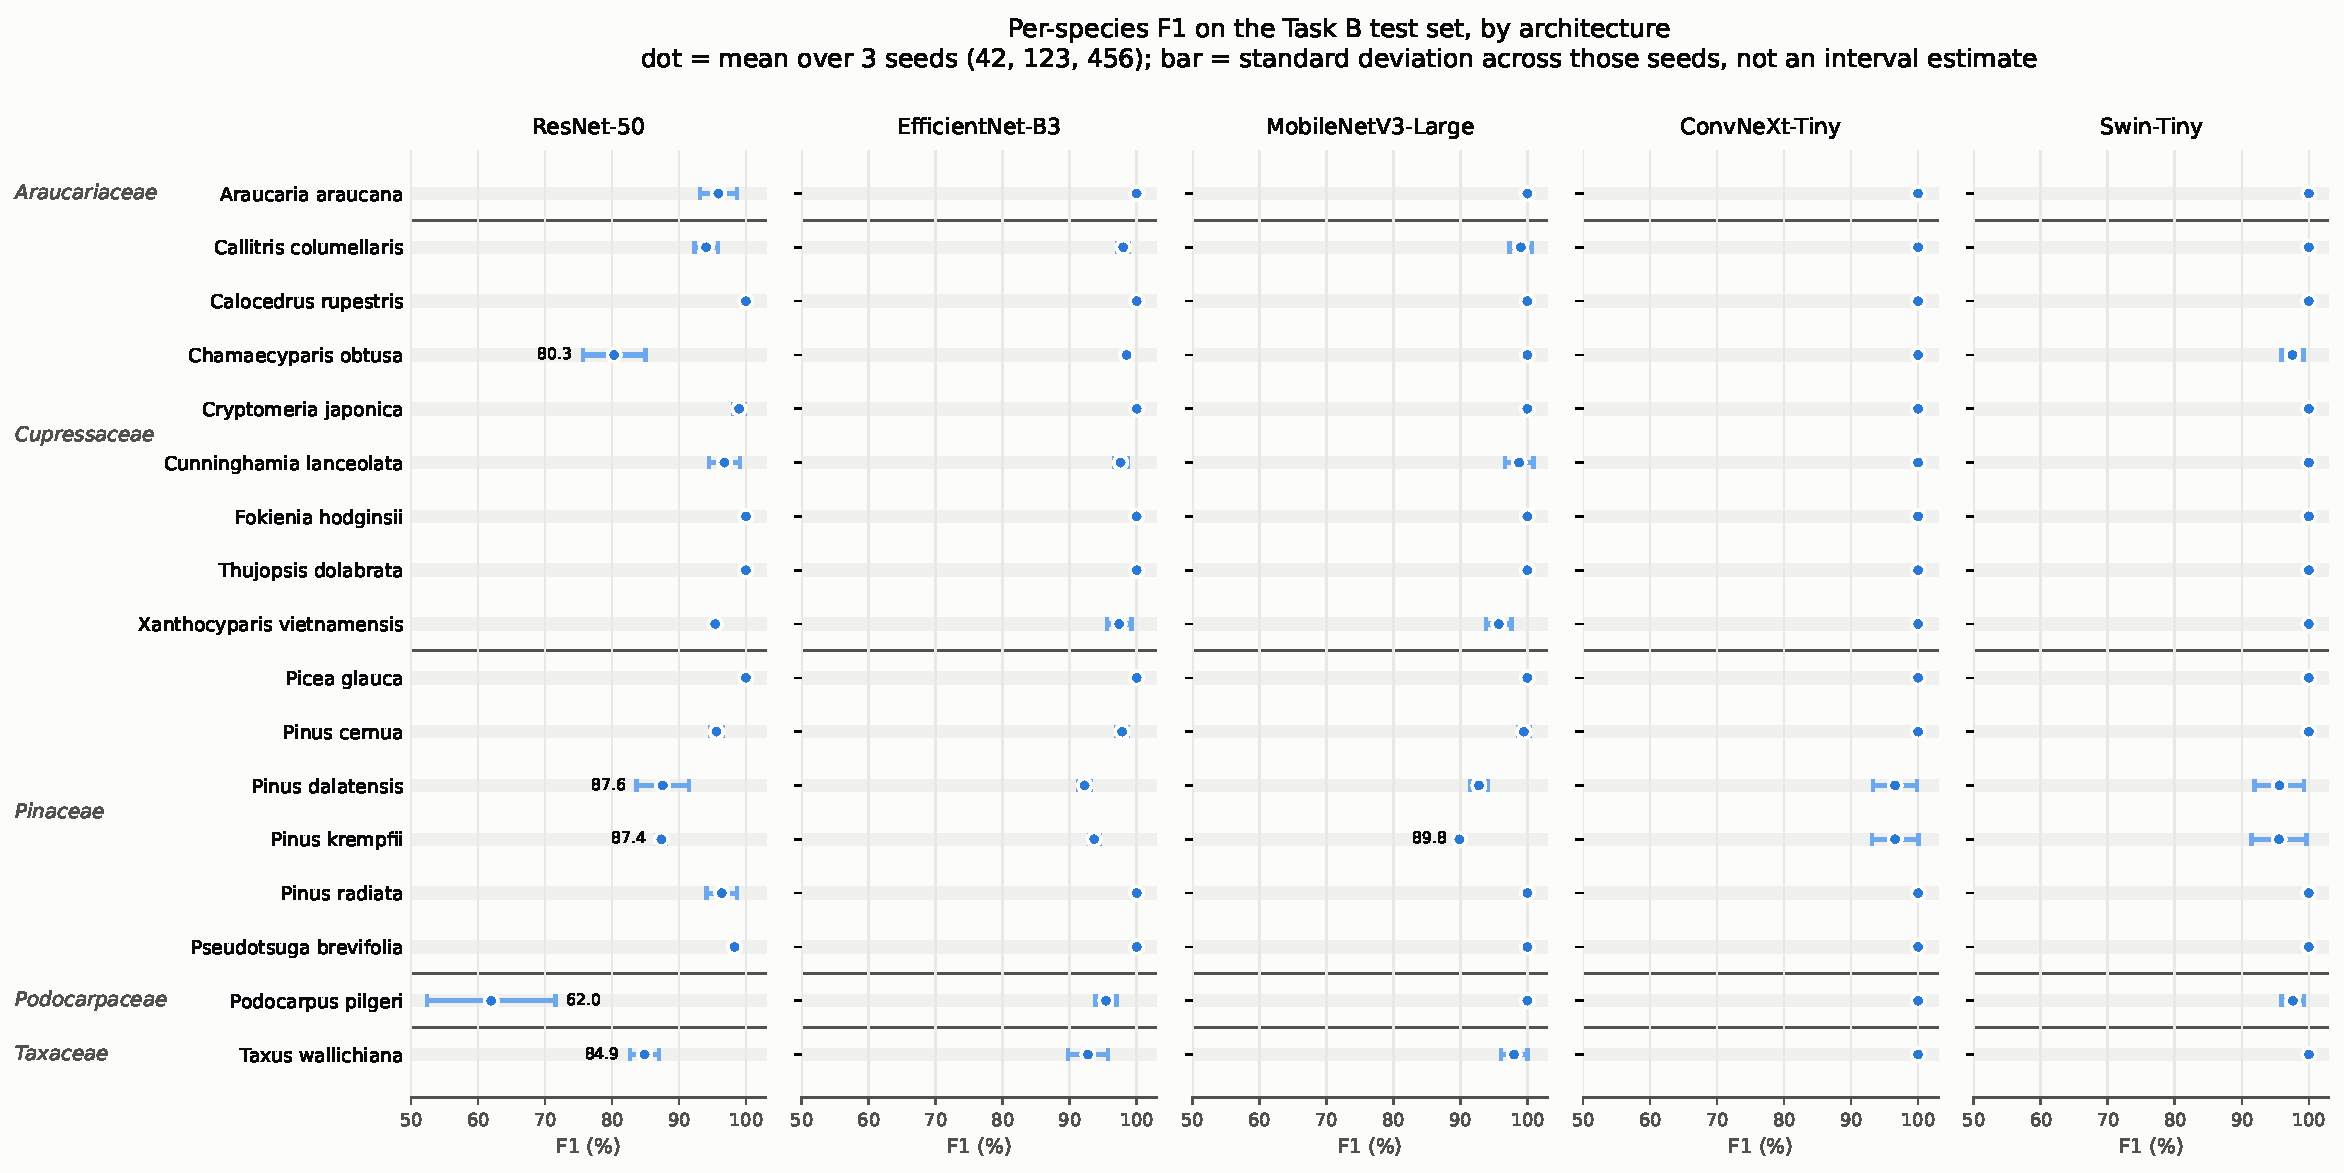
\includegraphics[width=\linewidth]{artifact/person3/per_class/fig_perclass_f1.pdf}
\caption{Per-species F1 on the Task~B test set, one panel per architecture.
Each dot is the mean over the three main seeds (42, 123, 456) and each bar is
the standard deviation across those seeds; the bar is a dispersion measure over
three runs and is not an interval estimate. Species are ordered by family, with
family blocks separated by horizontal rules and labelled at the left margin.
The horizontal axis is a position encoding and therefore does not start at
zero; values below 90\,\% are labelled directly. Architectures are separated
into panels rather than distinguished by colour, so that identity is carried by
position and panel title.}
\label{fig:perclass}
\end{figure}
